%
% Erstellt von Daniel Falkner
% daniel.falkner@akad.de
% 
\documentclass[xcolor=dvipsnames]{beamer}
\usepackage[T1]{fontenc}
\usepackage[utf8]{inputenc}
\usepackage[ngerman]{isodate}
\usepackage[justification=centering,figurename=Abb.]{caption}
\usepackage{listings}
\usepackage{color}


\definecolor{mygreen}{rgb}{0,0.6,0}
\definecolor{mygray}{rgb}{0.5,0.5,0.5}
\definecolor{mymauve}{rgb}{0.58,0,0.82}

\lstdefinelanguage{JavaScript}{
  keywords={break, case, catch, continue, debugger, default, delete, do, else, finally, for, function, if, in, instanceof, new, return, switch, this, throw, try, typeof, var, void, while, with},
  morecomment=[l]{//},
  morecomment=[s]{/*}{*/},
  morestring=[b]',
  morestring=[b]",
  sensitive=true
}

\lstdefinelanguage{CSS}
{morekeywords={color,background,margin, font, width, float, height, padding, box, opacity, border, right, top, shadow, radius, bottom},
sensitive=false,
morecomment=[l]{//},
morecomment=[s]{/*}{*/},
morestring=[b]",
} 

\lstset{ %
  backgroundcolor=\color{white},   % choose the background color; you must add \usepackage{color} or \usepackage{xcolor}
  basicstyle=\footnotesize,        % the size of the fonts that are used for the code
  breakatwhitespace=false,         % sets if automatic breaks should only happen at whitespace
  breaklines=true,                 % sets automatic line breaking
  captionpos=b,                    % sets the caption-position to bottom
  commentstyle=\color{mygreen},    % comment style
  deletekeywords={...},            % if you want to delete keywords from the given language
  escapeinside={\%*}{*)},          % if you want to add LaTeX within your code
  extendedchars=true,              % lets you use non-ASCII characters; for 8-bits encodings only, does not work with UTF-8
 % frame=single,                    % adds a frame around the code
  keepspaces=true,                 % keeps spaces in text, useful for keeping indentation of code (possibly needs columns=flexible)
  keywordstyle=\color{blue},       % keyword style
  language=Octave,                 % the language of the code
  morekeywords={*,...},            % if you want to add more keywords to the set
  numbers=left,                    % where to put the line-numbers; possible values are (none, left, right)
  numbersep=5pt,                   % how far the line-numbers are from the code
  numberstyle=\tiny\color{mygray}, % the style that is used for the line-numbers
  rulecolor=\color{black},         % if not set, the frame-color may be changed on line-breaks within not-black text (e.g. comments (green here))
  showspaces=false,                % show spaces everywhere adding particular underscores; it overrides 'showstringspaces'
  showstringspaces=false,          % underline spaces within strings only
  showtabs=true,                  % show tabs within strings adding particular underscores
  stepnumber=1,                    % the step between two line-numbers. If it's 1, each line will be numbered
  stringstyle=\color{mymauve},     % string literal style
  tabsize=2,                       % sets default tabsize to 2 spaces
  title=\lstname,                   % show the filename of files included with \lstinputlisting; also try caption instead of title
  belowskip= 0pt 
}

\usetheme{Warsaw}
\usecolortheme[named=OliveGreen]{structure}
\renewcommand\thempfootnote{\arabic{mpfootnote}}

\newcommand*{\Title}{Web 3.0: Daten sind das Öl des 21. Jahrhunderts} %Titel
\subtitle{Modul WIN03} %Untertitel
\newcommand*{\Author}{Daniel Falkner + Eugen Grinschuk} %Name
\institute{AKAD University} %Uni
\titlegraphic{
\includegraphics[scale=0.2]{akad_logo.png}} %Logo

\title{\Title}
\author{\Author}
\date{8.März.2014}

%Pdf Metainformationen
\subject{\Title}
\keywords{}

\begin{document}

%Titelseite
\begin{frame}
    \titlepage
\end{frame}

%Logo auf allen weiteren Folien
%\logo{
\includegraphics[scale=0.1]{akad_logo.png}}

%Inhaltsverzeichniss
\frame{\tableofcontents[hideothersubsections]} 


\section{Über uns}
\begin{frame} %%Eine Folie
  \frametitle{Über uns} %%Folientitel
  \begin{block}{Wer sind wir?}
	  \begin{itemize}
	  	\item AKAD Studenten - Bachelor of Science (Wirtschaftsinformatik)
	  \end{itemize}
  \end{block}
\end{frame}

\subsection{Daniel Falkner}
\begin{frame} %%Eine Folie
  \frametitle{Über uns} %%Folientitel
  \framesubtitle{Daniel Falkner} %%Fielenuntertitel
  \begin{block}{Daniel Falkner}
	  \begin{itemize}
  		\item T-Systems International GmbH - Telekom IT
  		\item IT-Architekt - System Analyst
		\item Projektleiter
		\item Proof of Concept Engineer
  		\item Debian Linux Administrator
	  \end{itemize}
  \end{block}
\end{frame}

\subsection{Eugen Grinschuk}
\begin{frame} %%Eine Folie
  \frametitle{Über uns} %%Folientitel
  \framesubtitle{Eugen Grinschuk} %%Fielenuntertitel
  \begin{block}{Eugen Grinschuk}
	  \begin{itemize}
  		\item T-Systems International GmbH
		\item IT-Architekt
  		\item Projektleiter
  		\item System Engineer
	  \end{itemize}
  \end{block}
\end{frame}

\section{Grundlagen}
\begin{frame} %%Eine Folie
  \frametitle{Grundlagen} %%Folientitel
        \tableofcontents[currentsection, hideothersubsections]
\end{frame}

\subsection{Big Data}
\begin{frame} %%Eine Folie
  \frametitle{Big Data} %%Folientitel
  \begin{block}{was ist Big Data und was macht man damit?}
	  \begin{itemize}
		\item Modebegriff
		\item große Menge an Daten (Tera - Peta - Exa - ???bytes)
	  	\item neue Technologien 
		\item Data-Mining
		\item Fraud-Detection
		\item Smart Metering
		\item Werbung
		\item Marktforschung
		\item Terrorismusbekämpfung
	  \end{itemize}
  \end{block}
\end{frame}


\subsection{Soziale Netzwerke allgemein}
\begin{frame} %%Eine Folie
  \frametitle{Soziale Netzwerke allgemein} %%Folientitel
  \begin{block}{eine Form von Online-Community}
	  \begin{itemize}
		\item Persönliches Profil
		\item Timeline	
	  	\item wir adden und liken
		\item public and "private" Messages
		\item Social Gaming
		\item Blog, Microblog
		\item Private oder Business Platformen
		\item API		
	  \end{itemize}
  \end{block}
\end{frame}



\subsection{Vorstellung Whatsapp}
\begin{frame} %%Eine Folie
  \frametitle{Vorstellung Whatsapp} %%Folientitel
  \begin{block}{Was ist Whatsapp}
	  \begin{itemize}
	  	\item Name ist ein Wortspiel (What's up?)
		\item Gründer Jan Koum und Brian Acton
		\item 450 Millionen Mitglieder im Frühjahr 2014
		\item 18 Milliarden Nachrichten pro Tag
		\item Multi Mobile Platform
		\item Basis XMPP Protokoll
		\item Mehr Möglichkeiten als eine einfache SMS
		\item Fotos, Video, Standort teilen
		\item immer wieder Sicherheitsprobleme
	  \end{itemize}
  \end{block}
\end{frame}


\subsection{Vorstellung Facebook}
\begin{frame} %%Eine Folie
  \frametitle{Vorstellung Facebook} %%Folientitel
  \begin{block}{Vorstellung Facebook}
	  \begin{itemize}
	  	\item größtes soziale Netzwerk mit über 1 Milliarde Nutzer
		\item Gründer Marc Zuckerberg
		\item Status, Ort, Fotos, Musik, Dokumente, Produkte, Freundschaften, Beziehungsstatus, etc. teilbar
		\item Social Media Marketing möglich (Facebook ads)
		\item Seiten für Privatperson, Unternehmen, Gruppe, Band, etc. können erstellt werden
		\item verschiedene Apps sind verfügbar
	  \end{itemize}
  \end{block}
\end{frame}

\subsection{Cookie-Tracking}
\begin{frame} %%Eine Folie
  \frametitle{Cookie-Tracking} %%Folientitel
  \begin{block}{Cookie-Tracking}
	  \begin{itemize}
	  	\item Nutzer kann wiedererkannt werden
		\item Cookie-Tracking-Dauer ist definierbar
		\item wird auf der Festplatte des PCs gespeichert
		\item Nutzerverhalten ermittelbar
		\item für Affiliate-Marketing sehr wichtig
	  \end{itemize}
  \end{block}
\end{frame}


\section{Hauptteil}
\begin{frame} %%Eine Folie
  \frametitle{Hauptteil} %%Folientitel
        \tableofcontents[currentsection, hideothersubsections]
\end{frame}

\subsection{Aktuelles Geschehen: Facebook kauft Whatsapp}
\begin{frame} %%Eine Folie
  \frametitle{Aktuelles Geschehen: Facebook kauft Whatsapp} %%Folientitel
  \begin{block}{das weltgrößte soziale Online-Netzwerk kauft den Rivalen WhatsApp}
	  \begin{itemize}
		\item 19 Milliarden Dollar, ca 14 Milliarden Euro
		\item Für den User kostet Whatsapp pro User/Jahr 1 Dollor
		\item Facebook zahlt pro User 42 Dollar
		\item es soll weiterhin werbefrei bleiben
		\item laut Mark Zuckerberg gibt es mehrere Wege damit Geld zu verdienen
	  \end{itemize}
  \end{block}
\end{frame}


\subsection{(Mögliche) Verwendbarkeit von Daten}
\begin{frame} %%Eine Folie
  \frametitle{(Mögliche) Verwendbarkeit von Daten} %%Folientitel
  \begin{block}{(Mögliche) Verwendbarkeit von Daten}
	  \begin{itemize}
	  	\item Hauptsächlich für personalisierte Werbung
		\item Userverhalten analysieren
		\item anbieten weiterer eigener Produkte
		\item Verbesserung der Webseite (Verweildauer, Service, Layout, etc.)
		\item Steigerung des Umsatzes
	  \end{itemize}
  \end{block}
  \begin{alertblock}{}
	  \begin{itemize}
		\item Datenschutz
		\item Verkauf von Userdaten
		\item unvorteilhafte Datenkorrelation
	  \end{itemize}
  \end{alertblock}
\end{frame}

\subsection{Vergleich zu Google}
\begin{frame} %%Eine Folie
  \frametitle{Vergleich zu Google} %%Folientitel
  \begin{block}{Vergleich zu Google}
	  \begin{itemize}
	  	\item größte Suchmaschine (>90\% Marktanteil in Deutschland, >60\% Marktanteil USA)
		\item größte Datenkrake überhaupt (0.5 Mio Server, Stand 2007, heute etwa 1 Mio)
		\item in nahezu jeder Branche verfügbar
		\item kennt seine Benutzer sehr genau
		\item bietet eigene Produkte wie Smartphones, Tablets, Betriebssystem, Browser, Cloud-Produkte, etc. an
		\item hat ebenfalls eigenes social network (Google +)
	  \end{itemize}
  \end{block}
\end{frame}

\subsubsection{Rechenzentrum}
\begin{frame}
  \frametitle{Rechenzentrum}
	\begin{figure}
		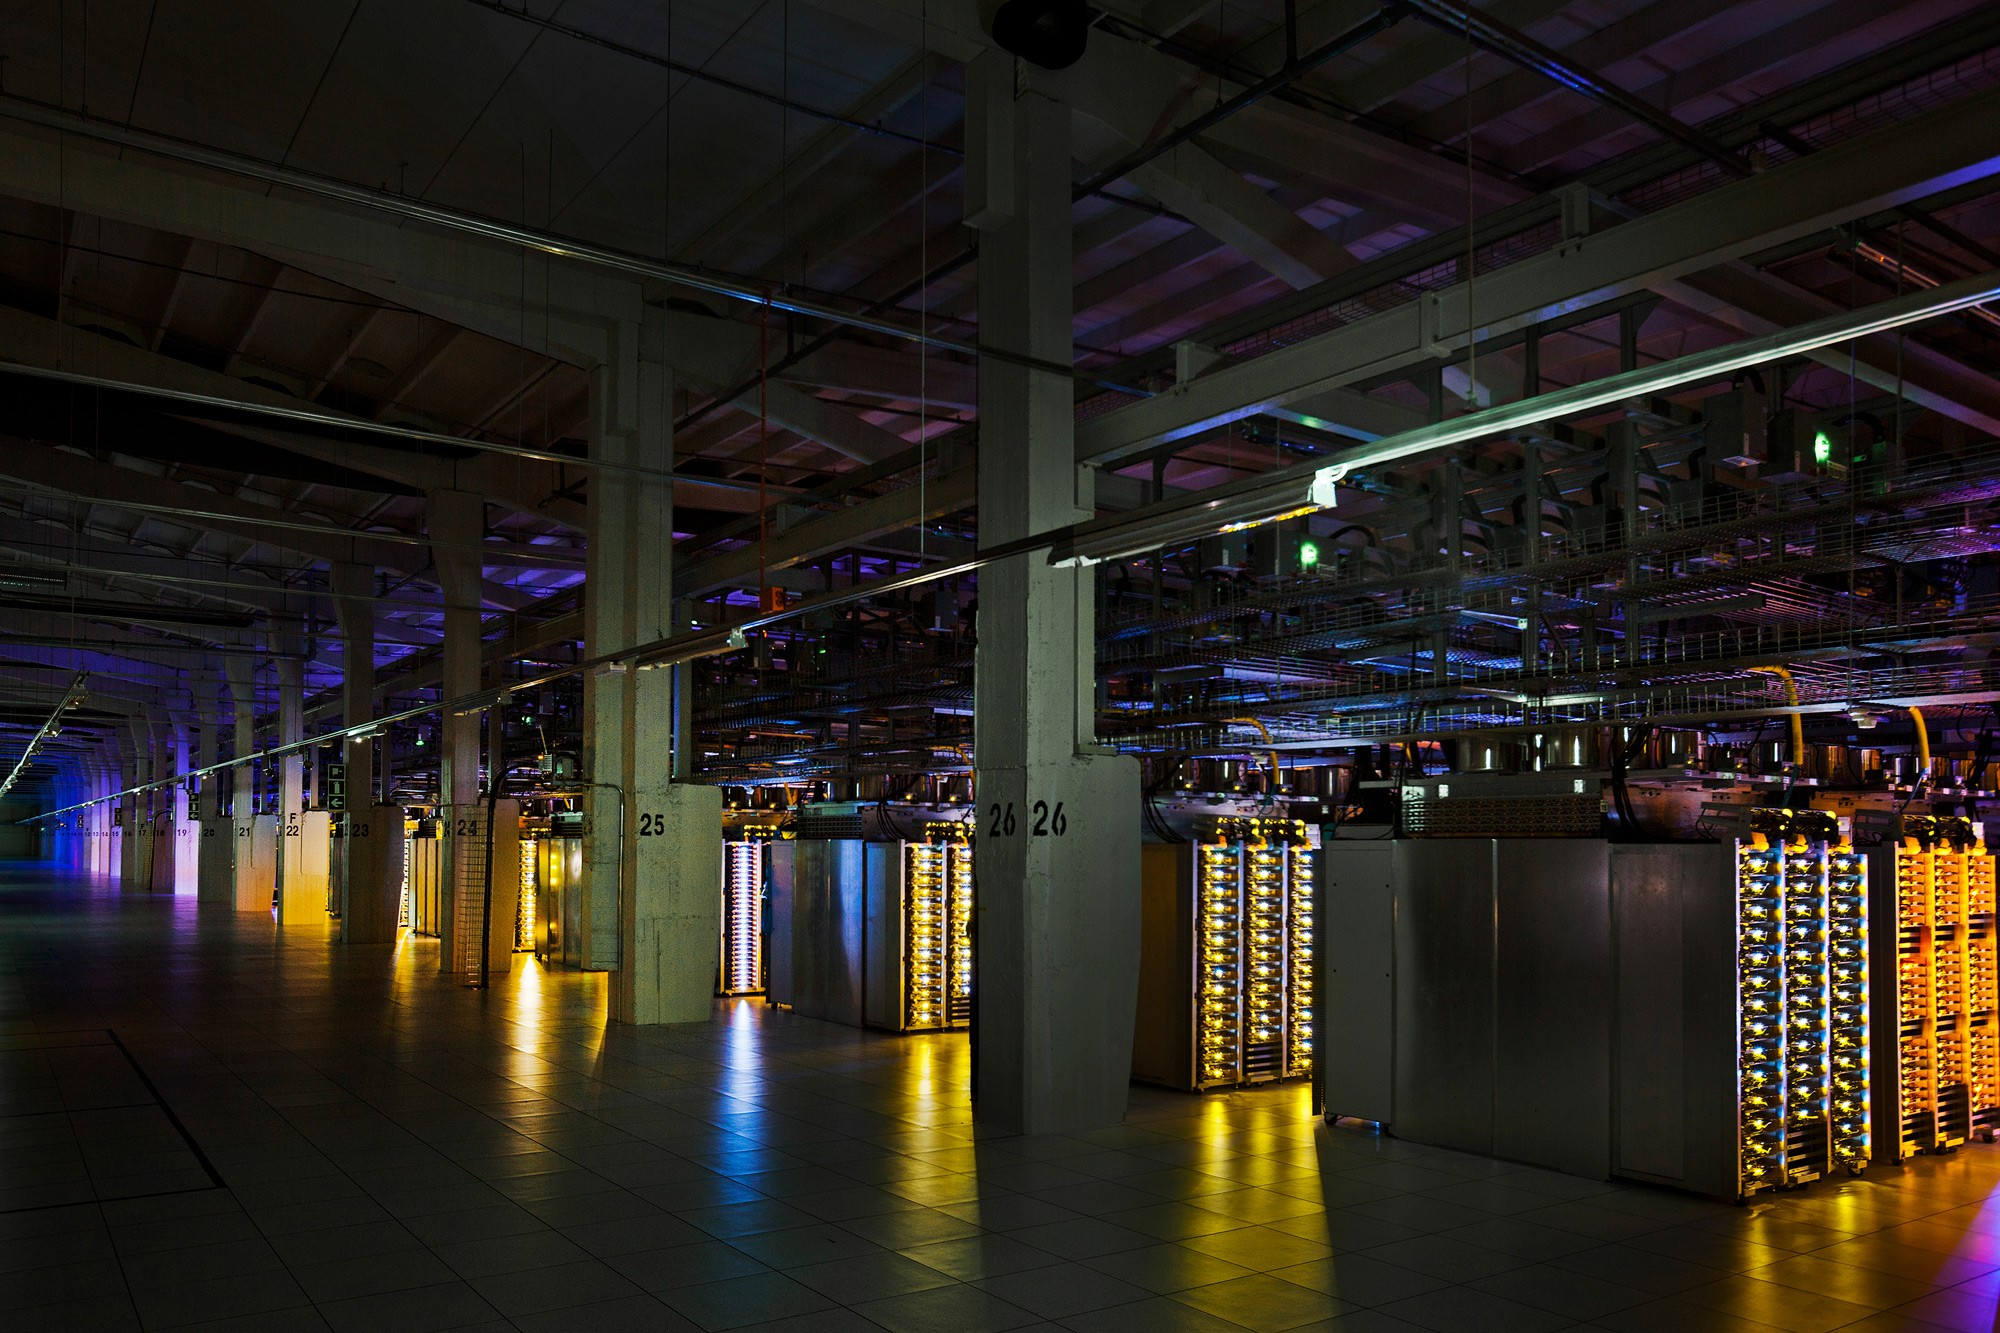
\includegraphics[scale=0.1]{LPP_016.jpg}
		\caption{Rechenzentrum \\ \tiny{\textcolor{gray}{\url{http://scr3.golem.de/screenshots/1210/Rechenzentren/thumb620/LPP_016.jpg}}}}
		\end{figure}
\end{frame}



\section{Anhang}
\begin{frame}
  \frametitle{Anhang} %%Folientitel
	\begin{block}{}	
		\begin{center}
			Vielen Dank für Ihre Aufmerksamkeit. \\
			Fragen?
		\end{center}	
	\end{block}
	\begin{block}{Links}	
		\begin{itemize}
			\item \url{https://github.com/derdanu/akad-win03-beamer}	
		\end{itemize}
	\end{block}
\end{frame}

\subsection{Quellen}
\begin{frame} %%Eine Folie
  \frametitle{Quellen} %%Folientitel
 	\begin{itemize}
		\item Google Deutschland \url{http://de.statista.com/statistik/daten/studie/167841/umfrage/marktanteile-ausgewaehlter-suchmaschinen-in-deutschland/}
		\item Google USA \url{http://www.seo-suedwest.de/454-suchmaschinen-marktanteile-us-mai-13.html
}
	\end{itemize}
\end{frame}




\end{document}


